\chapter{Introduzione alle smart card}
\label{chapter1}

%-----------------SECTION-----------------
\section{Cosa sono le smart card}
\label{intro}
Una smart card è un dispositivo hardware realizzato su un supporto di plastica in grado di elaborare e memorizzare dati, rispondendo anche ad elevati standard di sicurezza.

La prima idea di realizzare questo tipo di dispositivi è venuta nel 1968 a due inventori tedeschi: Jürgen Dethloff e Helmut Grötrupp. Da allora, grazie alle nuove tecnologie che hanno permesso di realizzare dispositivi sempre più piccoli e potenti, tale tecnologia si è diffusa proprio grazie alla sua versatilità.

Gli utilizzi delle smart card sono molteplici, dal settore bancario, a quello della telefonia, dell'identità, fino ad arrivare nel mondo del trasporto, con l'utilizzo di biglietti elettronici.
\cite{wiki_sc}

%------------------------------
\subsection{Caratteristiche  delle smart card}

Ci sono due criteri che permettono di classificare le smart card. Basandoci sulle potenzialità del circuito possiamo definire le smart card a sola memoria o a microprocessore. Invece il tipo di interfaccia di collegamento ci permette di distinguere tra smart card a contatto, senza contatto e con antenna e contattiera (ovvero a doppia interfaccia).

Le smart card a sola memoria hanno la capacità di memorizzare informazioni che possono essere lette successivamente, mentre quelle a microprocessore possono effettuare elaborazioni. Infine le smart card a contatto hanno dei pin connettori tramite i quali possono essere alimentate ed è possibile inviare e ricevere informazioni, mentre quelle senza contatto hanno a disposizione un'antenna che reagisce a un particolare campo elettromagnetico emesso da un dispositivo di lettura/scrittura.

Le smart card rispondono allo standard ISO 7816 che definisce le caratteristiche che devono avere le card a contatto, mentre altri standard sono usati per le card senza contatto (ISO 14443 e ISO 15693). Lo standard ISO 7816 sarà trattato più nel dettaglio nel paragrafo \ref{standard}.

Le smart card a microprocessore sono particolarmente utilizzate per conservare in maniera sicura una chiave privata. Grazie alla loro capacità di elaborazione sono in grado di ricevere una piccola quantità di dati (come ad esempio un hash di un documento) e restituirlo crittografato con la chiave privata contenuta al loro interno. In questo modo la chiave non ``esce" mai dal microprocessore, e quindi non può essere letta in alcun modo. Grazie a questa caratteristica le smart card costituiscono un elemento sicuro per la firma digitale di documenti.
\cite{wiki_sc}

%-----------SECTION------------
\section{Breve storia delle smart card}
Come accennato nel paragrafo \ref{intro}, l'idea di installare un chip elettronico su una scheda in plastica è venuta a due inventori tedeschi (Jürgen Dethloff e Helmut Grötrupp) nel 1968. Due anni dopo (nel 1970) è stato registrato il primo brevetto di smart card e nel 1976 si sono avute le prime card con microprocessore e memoria. Successivamente, nel 1979, l'azienda Motorola ha sviluppato la prima carta con chip sicuro per il settore bancario.

I primi test a larga scala delle smart card sono iniziati in Francia con i primi sportelli automatici, mentre negli stati uniti le smart card sono state inizialmente distribuiti ai lavoratori del settore agricolo. Ogni agricoltore ha ricevuto una card per la vendita delle arachidi. Una volta portato il raccolto presso un punto vendita autorizzato, i computer calcolavano la quantità del raccolto e la registravano sulle apposite card dei lavoratori.

Intanto in Europa al prima distribuzione in scala delle smart card è avvenuta ad opera dei Francesi con le card per le cabine telefoniche. La società Schlumberger è stata tra le prime ad implementare una struttura a chiave di cifratura pubblica per la gestione digitale dei certificati. Inoltre nel 1992 la Francia è stata la prima a realizzare delle card che richiedevano un PIN per essere utilizzate, introducendo le così dette  \textit{Carte Bleue} che si trattavano di carte di credito.

Un anno dopo, nel 1993, è nato il cosiddetto standard EMV (Europay MasterCard Visa) per l'utilizzo dei POS quando le varie compagnie hanno deciso di definire uno standard per le carte di credito in Europa. In America MasterCard ha iniziato ad accettare questo standard solo nel 2014.
\cite{history}

%-----------------SECTION-----------------
\section{Principali utilizzi delle smart card}
Oggigiorno le smart card sono vastamente utilizzate in una serie di ambiti e applicazioni differenti. In questa sezione sono elencati i principali utilizzi che vengono fatti attualmente.
%------------------------------
\subsection{Le smart card nella firma digitale}
\label{firma_digitale}
Come accennato nel paragrafo precedente, uno degli utilizzi delle smart card più frequente è quello nell'ambito della firma digitale.

La firma digitale è un insieme di metodi crittografici che servono a garantire l'autenticità di un messaggio trasmesso su canali non sicuri, offrendo al destinatario tre garanzie:
\begin{itemize}
    \item L'autenticazione del mittente.
    \item Il non ripudio di invio del messaggio da parte dell'utente.
    \item L'integrità del messaggio inviato.
\end{itemize}

La firma digitale si basa su un sistema di cifratura asimmetrica (ovvero che utilizza due chiavi, una pubblica e una privata). La chiave privata è utilizzata per ``firmare'' il file, mentre quella pubblica, disponibile a chiunque, per la verifica della validità della firma.

Il classico funzionamento di una firma digitale consiste in pochi semplici step:
\begin{enumerate}
    \item Tramite una funzione di hash viene generata una stringa identificativa univoca al file. File uguali generano la stessa stringa (se viene usata la stessa funzione di hash) ed ogni stringa identifica univocamente un file.
    \item La stringa generata con la funzione di hash viene crittografata usando la chiave privata. Una volta cifrata, la firma viene allegata al documento, che risulta firmato.
    \item Per verificare l'autenticità della firma e l'integrità del documento il ricevente può calcolare nuovamente la funzione di hash del file e decifrare la firma allegata usando la chiave pubblica del mittente. Se il documento non è stato alterato e la chiave pubblica usata per decifrare la firma corrisponde alla chiave privata usata dal mittente, allora la stringa di hash calcolata corrisponderà alla stringa decifrata. Ciò garantisce i tre parametri riportati sopra.
\end{enumerate}

La chiave pubblica è solitamente fornita da una Certification Autority (CA) che garantisce che si tratti effettivamente della chiave pubblica del mittente del messaggio.

Il ruolo che la smart card gioca nella firma digitale consiste nel conservare la chiave privata in un luogo sicuro. Il codice è, infatti, salvato sulla memoria del chip presente sulla card, che poi viene reso inaccessibile dall'esterno. Una volta collegata la card a un calcolatore, tramite un apposito lettore, al momento della firma viene inviato alla card la stringa identificativa del file. La scheda provvederà poi a crittografare la stringa e a restituire il risultato dell'elaborazione al PC che provvederà infine ad allegare la vera e propria firma al documento.
\cite{Wiki_fd}

%------------------------------
\subsection{Le smart card nella telefonia mobile}
\label{applet_sim}
Un altro utilizzo molto frequente delle smart card è quello nell'ambito della telefonia mobile.

Viene detta SIM (dall'inglese Subscriber Identity Module) una smart card che viene inserita in un telefono cellulare e utilizzata dagli operatori telefonici per conservare in modo sicuro il codice identificativo dei loro clienti (l'IMSI che corrisponde alla sigla inglese International Mobile Subscriber Identity).

Le caratteristiche tipiche di una smart card SIM sono riassunte nella tabella \ref{parametri_SIM}.

\begin{table}[h!]
\centering
\begin{tabular}{ |c|c| } 
 \hline
 Descrizione &  64K JavaCard 2.1.1 WIB1.3 USIM \\
 \hline
 Piattaforma & Atmel AT90SC25672RU \\ 
 \hline
 Architettura CPU & 8-bit AVR \\ 
 \hline
 Tecnologia & 0.15uM CMOS \\ 
 \hline
 ROM & 256KB \\
 \hline
 Memoria non volatile & 72 KB EEPROM \\
 \hline
 RAM & 6Kb \\
 \hline
 Frequenza operativa interna & 20-30 MHz \\
 \hline
 Tempo di vita & 500mila cicli di letture/scrittura \\
 \hline
 
\end{tabular}
\caption{Tabella dei parametri tipici di una smart card SIM \cite{secret_life}.}
\label{parametri_SIM}
\end{table}

L'utilizzo che viene fatto delle sim dagli operatori è quello di fornire vari servizi ai loro clienti e controllarne l'utilizzo.

La carta SIM non contiene in memoria il numero telefonico associato all'utente, ma solo il codice identificativo IMSI ed è compito dell'operatore associarlo ad un numero telefonico; grazie a ciò è possibile avere più SIM associate allo stesso numero o portare il proprio numero da un operatore a un altro.

La SIM è protetta da un codice PIN composto solitamente da 4 o 8 cifre, l'utente ha la facoltà di disabilitare la richiesta del codice ogni volta che la SIM viene alimentata oppure cambiare il codice fornito dall'operatore. Una volta che il codice PIN è stato sbagliato tre volte, la scheda si blocca e viene richiesto un codice di sblocco a 10 cifre, denominato PUK (PIN Unblocking Key) fornito dall'operatore. Se il codice PUK viene sbagliato 10 volte la scheda si blocca definitivamente e può essere sbloccata solo dall'operatore dopo aver provato di essere l'intestatario della SIM.

Il funzionamento della SIM è molto semplice. Una volta che l'operatore riconosce il codice presente sulla carta come valido e presente nel proprio database il dispositivo mobile viene agganciato alla rete e resta in attesa che l'utente richieda un particolare servizio. Una volta effettuata la richiesta, l'operatore verifica se il servizio può essere erogato controllando ad esempio le offerte attive e il credito disponibile e può decidere se accettare o rifiutare la richiesta.
\cite{Wiki_sim}

%------------------------------
\subsection{Le smart card nel settore bancario}
\label{carta_di_credito}
Un altro ambito nel quale le smart card sono ampiamente utilizzate è quello del settore bancario nel quale sono utilizzate per la realizzazione di carte di credito.

Le carte di credito sono dispositivi molto utilizzati per l'elaborazione di pagamenti e/o il trasferimento di denaro in quanto in grado di identificare l'utente utilizzatore e la banca emittente.

Inizialmente le carte di credito utilizzavano una banda magnetica per memorizzare il codice identificativo, tuttavia, per far fronte a esigenze sempre più stringenti sulla sicurezza e l'affidabilità di questi dispositivi, si è scelto di utilizzare un chip integrato rendendole, a tutti gli effetti, delle smart card. Inoltre un chip, oltre a conservare le informazioni della card in modo più sicuro, ha una memoria molto più ampia di quella che poteva avere una banda magnetica. Grazie a ciò, le card a micro chip possono offrire maggiori funzionalità delle card a banda magnetica, infatti vengono chiamate card "multi-applicazione".

Le dimensioni di una carta di credito sono definite dallo standard ISO/IEC 7810 ID01 e valgono 85,60 x 53,98 mm con uno spessore di 0,76 mm.

Alle carte di credito è sempre associato un codice PIN, che viene inserito ogni volta si voglia effettuare un pagamento.

Le carte di credito vengono principalmente utilizzate per effettuare pagamenti o prelevare denaro. Una transazione effettuata con carta di credito è un processo di autorizzazione tra tre enti:
\begin{itemize}
    \item L'Ente emittente, ovvero la società che emette la carta di credito. Questa società stipula un contratto con il titolare della carta che viene considerato suo cliente a tutti gli effetti.
    \item L'Ente esercente, ovvero il commerciante che aderisce a un circuito di pagamento offrendo ai propri clienti un metodo di pagamento alternativo al contante. Per aderire al circuito, l'esercente di rivolge a una società di gestione terminali che offre la vendita o l'affitto di dispositivi POS (Point of sale) tramite i quali l'esercente può elaborare i dati della carta di credito del proprio cliente.
    \item Il circuito di pagamenti, invece, è l'azienda che crea e gestisce una propria rete di comunicazione alla quale sono collegati i POS degli esercenti tramite la quale viaggiano le richieste di pagamento e le eventuali autorizzazioni.
\end{itemize}
Quindi la transazione avviene attraverso tre attori:
\begin{enumerate}
    \item Il \textit{titolare} della carta che si impegna a restituire i soldi della spesa all'emittente della carta secondo quanto stabilito nel contratto.
    \item Il \textit{fornitore} che eroga i servizi o i beni richiesti dal titolare della carta.
    \item L'\textit{istituto} emittente che si impegna a pagare il fornitore il prezzo stabilito drante la transazione a meno di eventuali canoni concordati in fase di stipula del contratto con il fornitore.
\end{enumerate}

Tra le principali tipologie di carte di credito la più comune è sicuramente la \textit{Carta di credito ``a saldo"}, fornita dalle banche a seguito dell'apertura di un conto corrente. Questa card da la possibilità di pagare tutte le spese effettuate in un mese solare in un'unica soluzione il mese successivo.

Un'altra tipologia di carta molto comune, sempre emessa dalle banche, è la cosiddetta \textit{Carta di credito rateale o rotativo} che permette di rateizzare i pagamenti della merce acquistata.

Le principali carte di credito sono:
\begin{itemize}
    \item American Express
    \item Diners
    \item Visa
    \item MasterCard
    \item JCB
    \item Discover Card
    \item China UnionPay
\end{itemize}

Inoltre la prima cifra del codice della card serve per identificare il circuito di appartenenza e per questo è sempre la stessa per ogni carta appartenente al medesimo circuito.
\begin{itemize}
    \item Diners: 3
    \item American Express: 3
    \item Visa: 4
    \item MasterCard: 5
    \item Discover Card: 6
\end{itemize}

L'unico rischio in cui si può incorrere quando si ha una carta di credito consiste nella possibilità di smarrimento e/o clonazione dei codici usati per l'autenticazione e l'autorizzazione del pagamento. In caso di furto o smarrimento è sempre possibile bloccare la carta effettuando la richiesta presso il proprio fornitore.
\cite{Wiki_cc}

%------------------------------
\subsection{Le smart card nell'identificazione}
\label{carta_identita_elettronica}
A luglio 2016 è partita, in Italia, la sostituzione della carta d'identità cartacea con quella elettronica.

Oltre a cambiare le dimensioni e il materiale dal quale è costituito, il documento è stato anche munito di un microprocessore a radio frequenza, rendendolo di fatto una smart card contactless.

I dati contentuti all'interno del chip sono i seguenti:
\begin{itemize}
    \item Comune emettitore
    \item Nome del titolare
    \item Cognome del titolare
    \item Luogo e data di nascita
    \item Sesso
    \item Statura
    \item Cittadinanza
    \item Immagine della firma del titolare
    \item Validità per l’espatrio
    \item Fotografia
    \item Immagini di 2 impronte digitali (un dito della mano destra e un dito della mano sinistra)
    \item Nome e cognome del padre e della madre (nel caso di un minore)
    \item Codice fiscale
    \item Estremi dell’atto di nascita
    \item Indirizzo di residenza
    \item Comune di iscrizione AIRE (per i cittadini residenti all’estero)
    \item Codice fiscale sotto forma di codice a barre
\end{itemize}

L'accesso ai dati presenti sul microprocessore è effettuato attraverso la tecnologia NFC  (Near Field Communication), ciò permette alla carta di essere letta non solo da appositi lettori, ma anche dai più moderni smartphone dotati di lettori NFC.

L'applicazione tramite la quale viene effettuata la verifica del documento è la stessa presente anche nei passaporti moderni, denominata ``ICAO MRTD" (International Civil Aviation Organization - Machine Readable Travel Documents). L'applicazione contiene tutti i dati anagrafici dell'utente che sono firmati digitalmente dal Ministero dell’Interno prima che la carta venga prodotta presso l’Istituto Poligrafico e Zecca dello Stato.

La sicurezza dei dati è garantita dal fatto che la loro lettura è consentita solo a chi può leggere le informazioni stampate fisicamente sulla carta. Questo perchè sulla card è presente una chiave di accesso richiesta per la lettura elettronica (nel CAN – Card Access Number o nell’ MRZ – Machine Readable Zone). Invece, per l'accesso ai dati più sensibili, come le impronte digitali, sono richieste ulteriori autorizzazioni date a specifici organi come le forze di Polizia. Questo, insieme al fatto che la conversazione tra lettore e carta è cifrata, fa sì che le informazioni non possono essere lette all'insaputa dell'utente e blocca anche tentativi di intercettazione della comunicazione.
\cite{cie}

\subsubsection{Esempio di scansione di una carta d'identità}
In questa breve sezione si mostrerà come venga utilizzata la tecnologia NFC per la lettura della smart card presente all'interno di una carta d'identità tramite l'applicazione \textit{IDEA - Identity Easy Access} disponibile gratuitamente sul Google Play store per tutti gli smartphone Android dotati di lettore NFC.

Come primo passaggio, l'applicazione ha bisogno di leggere il codice di accesso presente sul retro della carta, ciò può essere fatto manualmente o mediante l'utilizzo della fotocamera. Questo processo è mostrato nella figura \ref{fig:leggi_codice}

\begin{figure}[h!]
  \centering
  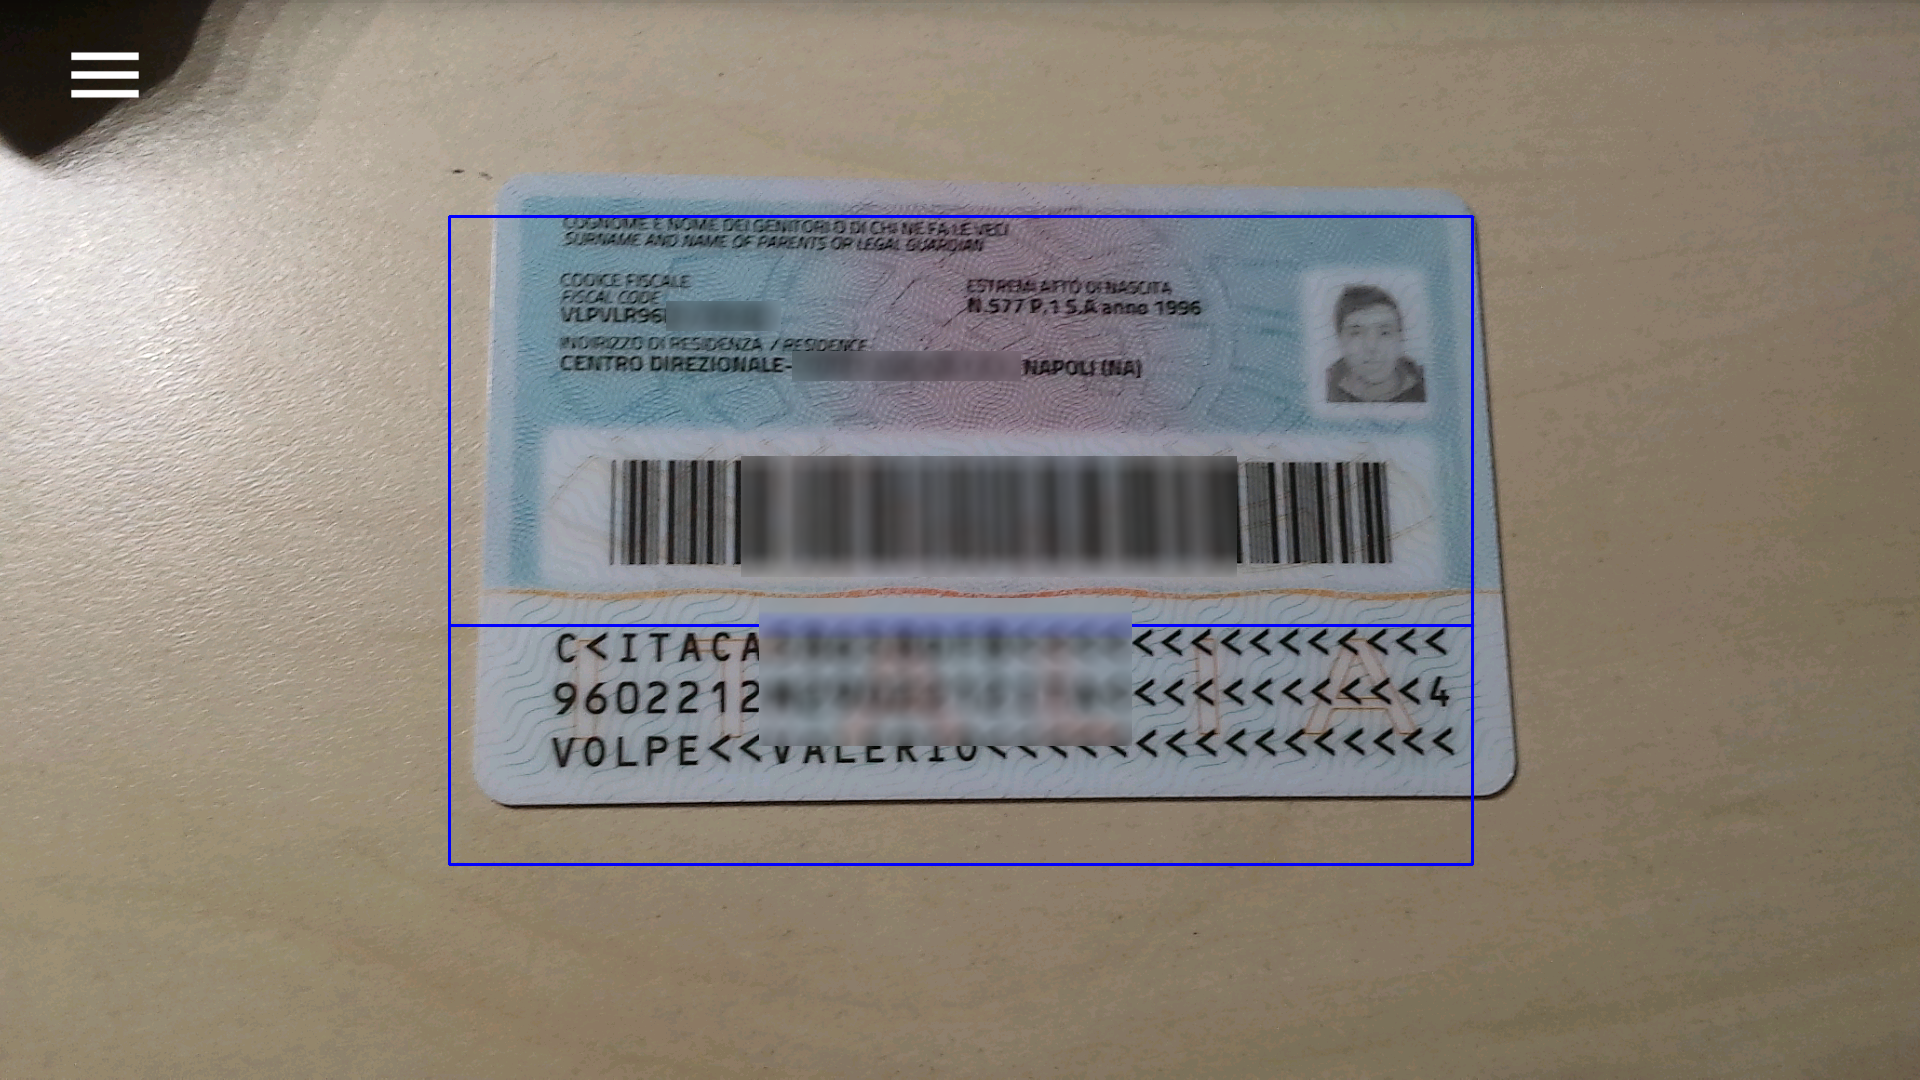
\includegraphics[width=300pt]{pictures/foto_carta.png}
  \caption{Lettura del codice di accesso tramite la fotocamera.}
  \label{fig:leggi_codice}
\end{figure}

Una volta fatto ciò è possibile avvicinare la carta al lettore NFC per far avvenire la richiesta e la comunicazione dei dati. Come mostrato nella figura \ref{fig:leggi_carta}.

\begin{figure}[h!]
  \centering
  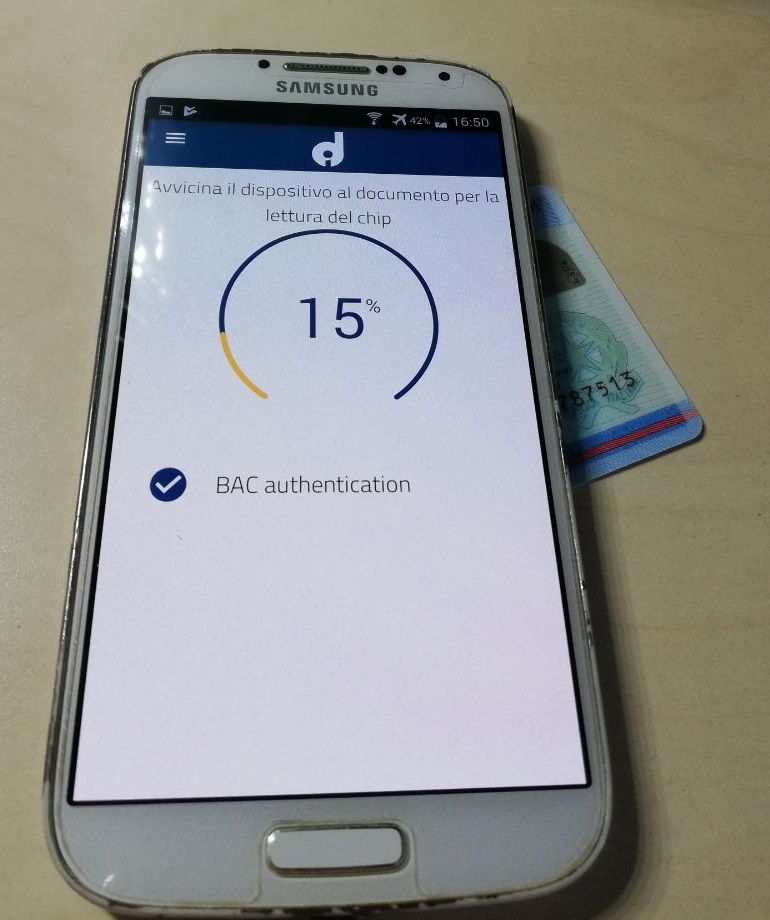
\includegraphics[width=200pt]{pictures/lettura_carta.jpg}
  \caption{Lettura della carta tramite NFC.}
  \label{fig:leggi_carta}
\end{figure}

Una volta terminata l'operazione è possibile vedere i dati che possono essere letti elettronicamente. Come si vede nella figura \ref{fig:carta_letta}, i dati che possono essere letti sono: il numero del documento, il nome, il cognome, il sesso, la data di nascita, la scadenza del documento e la foto del titolare, è inoltre possibile anche verificare l'autenticità del documento.

\begin{figure}[h!]
  \centering
  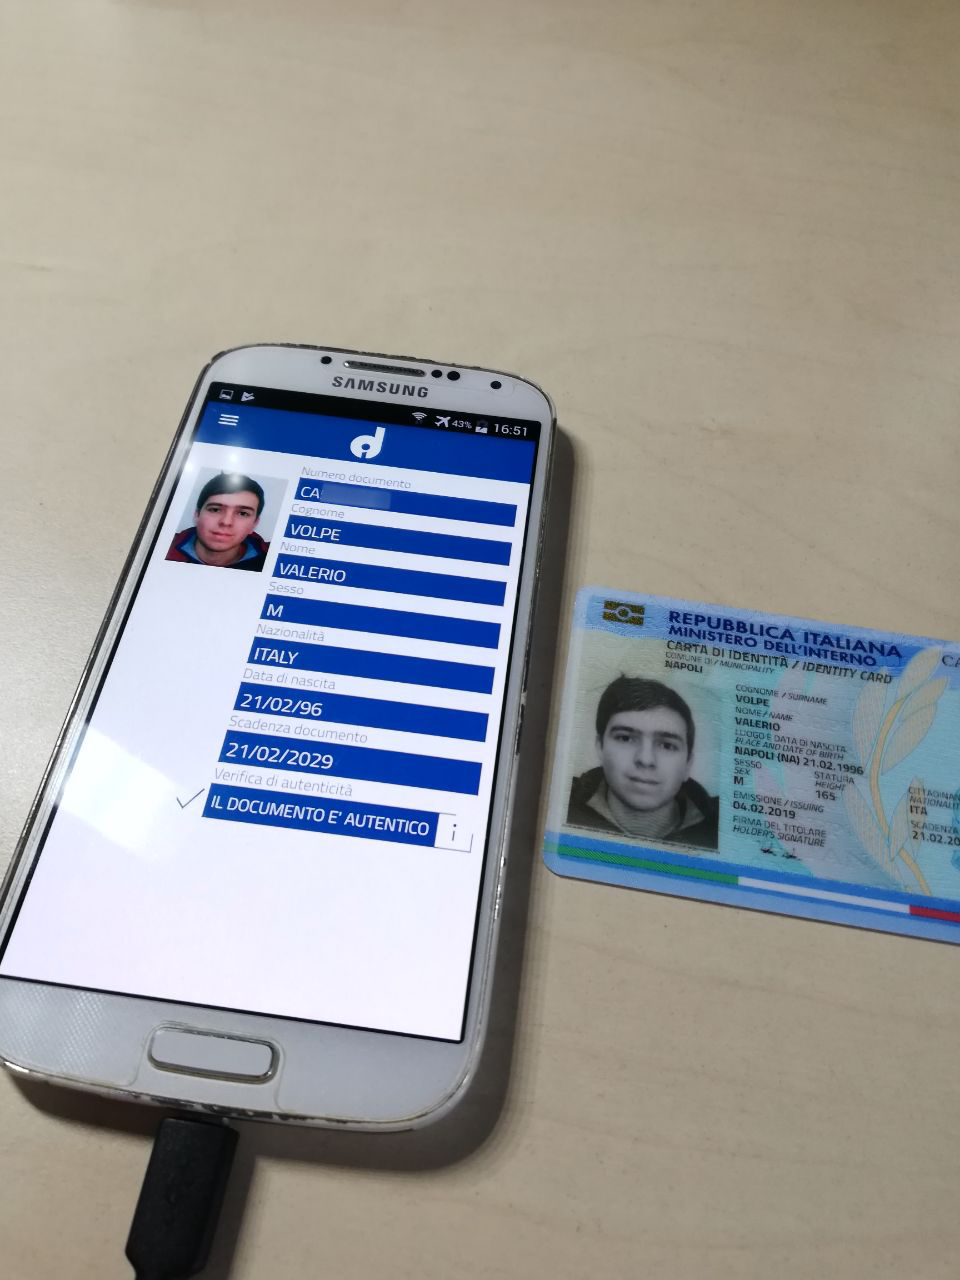
\includegraphics[width=250pt]{pictures/carta_letta.jpg}
  \caption{I dati letti elettronicamente dalla carta.}
  \label{fig:carta_letta}
\end{figure}
